%definira klasu dokumenta 
\documentclass[12pt]{report} 

%prostor izmedu naredbi \documentclass i \begin{document} se zove uvod. U njemu se nalaze naredbe koje se odnose na cijeli dokument

%osnovni LaTex ne može riješiti sve probleme, pa se koriste različiti paketi koji olakšavaju izradu željenog dokumenta
\usepackage[croatian]{babel} 
\usepackage{amssymb}
\usepackage{amsmath}
\usepackage{txfonts}
\usepackage{mathdots}
\usepackage{titlesec}
\usepackage{array}
\usepackage{lastpage}
\usepackage{etoolbox}
\usepackage{tabularray}
\usepackage{color, colortbl}
\usepackage{adjustbox}
\usepackage{geometry}
\usepackage[classicReIm]{kpfonts}
\usepackage{hyperref}
\usepackage{fancyhdr}

\usepackage{float}
\usepackage{setspace}
\restylefloat{table}


\patchcmd{\chapter}{\thispagestyle{plain}}{\thispagestyle{fancy}}{}{} %redefiniranje stila stranice u paketu fancyhdr

%oblik naslova poglavlja
\titleformat{\chapter}{\normalfont\huge\bfseries}{\thechapter.}{20pt}{\Huge}
\titlespacing{\chapter}{0pt}{0pt}{40pt}


\linespread{1.3} %razmak između redaka

\geometry{a4paper, left=1in, top=1in,}  %oblik stranice

\hypersetup{ colorlinks, citecolor=black, filecolor=black, linkcolor=black,	urlcolor=black }   %izgled poveznice


%prored smanjen između redaka u nabrajanjima i popisima
\newenvironment{packed_enum}{
	\begin{enumerate}
		\setlength{\itemsep}{0pt}
		\setlength{\parskip}{0pt}
		\setlength{\parsep}{0pt}
	}{\end{enumerate}}

\newenvironment{packed_item}{
	\begin{itemize}
		\setlength{\itemsep}{0pt}
		\setlength{\parskip}{0pt}
		\setlength{\parsep}{0pt}
	}{\end{itemize}}




%boja za privatni i udaljeni kljuc u tablicama
\definecolor{LightBlue}{rgb}{0.9,0.9,1}
\definecolor{LightGreen}{rgb}{0.9,1,0.9}

%Promjena teksta za dugačke tablice
\DefTblrTemplate{contfoot-text}{normal}{Nastavljeno na idućoj stranici}
\SetTblrTemplate{contfoot-text}{normal}
\DefTblrTemplate{conthead-text}{normal}{(Nastavljeno)}
\SetTblrTemplate{conthead-text}{normal}
\DefTblrTemplate{middlehead,lasthead}{normal}{Nastavljeno od prethodne stranice}
\SetTblrTemplate{middlehead,lasthead}{normal}

%podesavanje zaglavlja i podnožja

\pagestyle{fancy}
\lhead{Programsko inženjerstvo}
\rhead{BytePit}
\lfoot{Rade}
\cfoot{stranica \thepage/\pageref{LastPage}}
\rfoot{\today}
\renewcommand{\headrulewidth}{0.2pt}
\renewcommand{\footrulewidth}{0.2pt}


\begin{document} 
	
	
	
	\begin{titlepage}
		\begin{center}
			\vspace*{\stretch{1.0}} %u kombinaciji s ostalim \vspace naredbama definira razmak između redaka teksta
				\LARGE Programsko inženjerstvo\\
			\large Ak. god. 2023./2024.\\
			
			\vspace*{\stretch{3.0}}
			
			\huge BytePit\\
			\Large Dokumentacija, Rev. \textit{1}\\
			
			\vspace*{\stretch{12.0}}
			\normalsize
			Grupa: \textit{Rade}\\
			Voditelj: \textit{Marko Bolt}\\
			
			
			\vspace*{\stretch{1.0}}
			Datum predaje: \textit{17. 11. 2023.}\\
	
			\vspace*{\stretch{4.0}}
			
			Nastavnik: \textit{Hrvoje Nuić}\\
		
		\end{center}

	
	\end{titlepage}

	
	\tableofcontents


	\chapter{Dnevnik promjena dokumentacije}
		
				
		
		\begin{longtblr}[
				label=none
			]{
				width = \textwidth, 
				colspec={|X[2]|X[13]|X[3]|X[3]|}, 
				rowhead = 1
			}
			\hline
			\textbf{Rev.}	& \textbf{Opis promjene/dodatka} & \textbf{Autori} & \textbf{Datum}\\[3pt] \hline
			0.1 & Napravljen predložak.	& Marko Bolt & 04.11.2023. 		\\[3pt] \hline 
			0.2 & Napravljen opis projekta & Marko Bolt & 05.11.2023.\\[3pt] \hline	
			0.3 & Napravljeni funkcionalni zahtjevi & Jakov Vinožganić Teo Radolović & 09.11.2023.\\[3pt] \hline	
			0.4 & Napravljeni obrasci uporabe & Filip Bernt & 10.11.2023.\\[3pt] \hline
			0.5 & Napravljeni sekvencijski dijagrami & Filip Bernt Fran Sipić & 10.11.2023.\\[3pt] \hline	
			0.6 & Napravljeni ostali zahtjevi & Jure Franjković & 12.11.2023.\\[3pt] \hline	
			0.7 & Napravljena arhitektura i dizajn sustava & Jure Franjković & 13.11.2023.\\[3pt] \hline	
			0.8 & Napravljen opis baze podataka & Filip Bernt Fran Sipić & 14.11.2023.\\[3pt] \hline	
			0.9 & Napravljen dijagram razreda & Jure Franjković & 15.11.2023.\\[3pt] \hline	
			1.0 & Napravljena finalna inačica za prvi ciklus & Filip Bernt & 17.11.2023.\\[3pt] \hline	
			1.1 & Napravljen dijagram komponenti & Filip Bernt & 19.12.2023.\\[3pt] \hline	
		\end{longtblr}
	
	
	\chapter{Opis projektnog zadatka}
		
		\textbf{\textit{dio 1. revizije}}\\
		
		Aplikacija ByteBit inovativno je rješenje namijenjeno provjeri 
		programerskih vještina, omogućavajući korisnicima sudjelovanje u 
		programskim natjecanjima i vježbanje rješavanja zadataka. Aplikacija 
		se može implementirati kao web ili desktop platforma koristeći 
		objektno-orijentirane programerske jezike, sa podrškom za kompilaciju
		i evaluaciju rješenja u najmanje jednom programskom jeziku.\\

		Glavne funkcionalnosti aplikacije uključuju:
		\begin{packed_item}
    	\item \textbf{Pregledavanje zadataka i kalendar natjecanja:} 
		Korisnici mogu pregledavati dostupne zadatke i kalendar natjecanja, 
		što omogućava planiranje sudjelovanja i pripremu.
    	\item \textbf{Profili korisnika:} Natjecatelji imaju profile s 
		prikazom statistika njihovih rezultata, uključujući broj točno 
		riješenih i isprobanih zadataka, kao i pehare za osvojena natjecanja.
		Profili voditelja sadrže informacije o učitanim zadacima i 
		organiziranim natjecanjima.
 		\item \textbf{Registracija korisnika:} Registracija zahtijeva 
		osnovne podatke kao što su korisničko ime, fotografija, lozinka, 
		ime, prezime i email adresa. Administrator potvrđuje registraciju,
		a u slučaju voditelja natjecanja potrebna je i dodatna verifikacija.
    	\item \textbf{Natjecanja:} Početkom natjecanja, zadaci postaju 
		vidljivi aktivnim natjecateljima. Nakon završetka, zadaci su
		dostupni svima. Postoji mogućnost slanja datoteka s programskim
		kodom i objavljivanje rang lista po bodovima, uzimajući u
		obzir vrijeme i točnost rješenja.
    	\item \textbf{Prikaz rješenja:} Natjecatelji mogu vidjeti 
		rješenja drugih natjecatelja nakon natjecanja, dok su tijekom 
		natjecanja vidljiva samo ako su sami točno riješili zadatak.
    	\item \textbf{Vježbanje:} Natjecatelji mogu vježbati zadatake i 
		učitavati rješenja, s automatskom provjerom točnosti i vremenskih ograničenja.
   		\item \textbf{Virtualna natjecanja:} Natjecatelji mogu stvoriti 
		vlastita virtualna natjecanja odabirom prošlih natjecanja ili 
		nasumičnim odabirom zadataka, a rezultati se uspoređuju s originalnim.
    	\item \textbf{Uloga voditelja:} Voditelji imaju mogućnost učitavanja 
		novih zadataka, organiziranja natjecanja, i odabira zadataka koji će 
		biti aktivni tijekom natjecanja, uz mogućnost uređivanja vlastitih zadataka.
   		\item \textbf{Administrativne funkcije:} Administratori imaju ovlasti 
		za upravljanje korisničkim računima i uređivanjem svih zadataka i 
		natjecanja, bez mijenjanja prethodno ostvarenih rezultata.\\
		\end{packed_item}


		Trenutno postoje brojne platforme poput Codeforces, LeetCode,
		HackerRank i drugih koje nude slične funkcionalnosti. Razlike
		u odnosu na BytePit bi se mogle ogledati u specifičnostima kao
		što su lokalizacija (jezik i regionalni fokus), specijalizacija
		za određene programerske jezike ili tehnologije, ili u razini
		personalizacije korisničkog iskustva.
		Slična rješenja i razlike:
		\begin{packed_item}
			\item \textbf{Codeforces}: Fokusira se na konkurentno programiranje s
			redovitim natjecanjima. BytePit bi mogao uključivati više edukativnih
			resursa i prilagodljiva virtualna natjecanja.
			\item \textbf{LeetCode}: Specijaliziran za pripremu tehničkih intervjua.
			BytePit može nuditi širi raspon zadatka, uključujući one van konteksta intervjua.
			\item \textbf{HackerRank}: Osim izazova u programiranju, nudi i podršku
			za tvrtke u regrutiranju. BytePit bi mogao dodati vrednost kroz specifične
			profile natjecanja i detaljnu statistiku.Sličan koncept, ali s fokusom na
			poslovne korisnike. BytePit bi mogao biti više usmjeren na edukaciju i natjecanja.\\
		\end{packed_item}


		BytePit bi mogao privući širok spektar korisnika, od početnika u programiranju 
		koji traže mjesto za učenje i prakticiranje, do iskusnih programera koji žele 
		oštriti svoje vještine ili sudjelovati u natjecanjima, te edukativnih institucija 
		koje traže platformu za organiziranje natjecanja ili kao alat u nastavi. Ova 
		raznolikost korisnika stvara dinamično okruženje u kojem se znanje i iskustvo 
		neprestano razmjenjuju, pružajući beskrajne mogućnosti za učenje i napredak. 
		S jedne strane, početnici imaju priliku učiti kroz praksu, rješavajući stvarne 
		probleme i dobivajući povratne informacije od iskusnijih kolega. S druge strane, 
		iskusni programeri mogu se suočavati s izazovnijim problemima i sudjelovati u 
		zahtjevnijim natjecanjima, što ih stavlja u poziciju mentora, potičući ih na 
		daljnji razvoj i dijeljenje znanja. Edukativne institucije mogu koristiti BytePit 
		za stvaranje prilagođenih tečajeva i kurikuluma, pružajući studentima praktično 
		iskustvo koje je ključno za njihov razvoj. Poslodavci koji traže talentirane 
		programere mogli bi koristiti platformu za identifikaciju potencijalnih kandidata, 
		provodeći natjecanja ili izazove koji služe kao dio procesa zapošljavanja ili kroz 
		analizu rješenja i pristupa problemima koje programeri koriste na platformi.
		\\

		BytePit bi trebao biti projektiran s mogućnostima prilagodbe, što bi uključivalo 
		konfigurabilne module za natjecanja, personalizirane profile korisnika, i fleksibilan 
		sustav ocjenjivanja. Prilagodba omogućava korisnicima da kreiraju jedinstveno 
		iskustvo koje odgovara njihovim specifičnim potrebama i stilu učenja ili rada. 
		Personalizirani profili omogućavaju korisnicima da predstave svoje vještine i 
		postignuća, kao i da prate svoj napredak kroz različite metrike i statistike. 
		Fleksibilan sustav ocjenjivanja omogućava različite forme evaluacije, od standardnog 
		bodovanja do složenih algoritama koji mogu vrednovati efikasnost koda ili kreativno 
		rješavanje problema. Ovo omogućava platformi da raste i evoluira zajedno sa svojim 
		korisničkim bazama i tehnološkim trendovima, ostajući relevantna i privlačna za 
		široki spektar korisnika, od individualaca i obrazovnih institucija do korporacija 
		i tehničkih zajednica.
		\\

		Opseg projekta uključuje dizajniranje i implementaciju korisničkih sučelja, koje 
		moraju biti intuitivna i pristupačna, osiguravajući ugodno iskustvo za sve korisnike, 
		neovisno o njihovom tehničkom znanju ili iskustvu u programiranju. Back-end servisi 
		za upravljanje bazom podataka moraju biti robustni i optimizirani za brzu obradu 
		upita, što je ključno za održavanje visoke performanse platforme čak i pod velikim 
		opterećenjem. Sustav za evaluaciju koda mora biti precizan i pouzdan, sposoban za 
		brzo i efikasno procjenjivanje raznovrsnih programskih rješenja koja korisnici 
		predaju. Sustav za autentifikaciju i autorizaciju korisnika treba osigurati da su 
		svi podaci sigurni i da pristup platformi
		\\

		Nadogradnje projekta mogu uključivati:
		\begin{packed_item}
			\item Integraciju s vanjskim servisima poput GitHub-a za uvoz postojećeg koda.
			\item Implementaciju naprednijih algoritama za detekciju plagijata.
			\item Proširenje podrške za više programskih jezika i tehnoloških okvira.
			\item Razvoj mobilne aplikacije za pristup platformi.
			\item Uvođenje umjetne inteligencije za personalizirane preporuke zadataka
			na temelju korisnikovih prethodnih aktivnosti i uspjeha.
			\item "Gamification" sustav za nagrađivanje korisnika za postignuća i napredak.
		\end{packed_item}


		\eject
		
		\section{Primjeri u \LaTeX u}
		
		\textit{Ovo potpoglavlje izbrisati.}\\

		U nastavku se nalaze različiti primjeri kako koristiti osnovne funkcionalnosti \LaTeX a koje su potrebne za izradu dokumentacije. Za dodatnu pomoć obratiti se asistentu na projektu ili potražiti upute na sljedećim web sjedištima:
		\begin{itemize}
			\item Upute za izradu diplomskog rada u \LaTeX u - \url{https://www.fer.unizg.hr/_download/repository/LaTeX-upute.pdf}
			\item \LaTeX\ projekt - \url{https://www.latex-project.org/help/}
			\item StackExchange za Tex - \url{https://tex.stackexchange.com/}\\
		
		\end{itemize} 	


		
		\noindent \underbar{podcrtani tekst}, \textbf{podebljani tekst}, 	\textit{nagnuti tekst}\\
		\noindent \normalsize primjer \large primjer \Large primjer \LARGE {primjer} \huge {primjer} \Huge primjer \normalsize
				
		\begin{packed_item}
			
			\item  primjer
			\item  primjer
			\item  primjer
			\item[] \begin{packed_enum}
				\item primjer
				\item[] \begin{packed_enum}
					\item[1.a] primjer
					\item[b] primjer
				\end{packed_enum}
				\item primjer
			\end{packed_enum}
			
		\end{packed_item}
		
		\noindent primjer url-a: \url{https://www.fer.unizg.hr/predmet/proinz/projekt}
		
		\noindent posebni znakovi: \# \$ \% \& \{ \} \_ 
		$|$ $<$ $>$ 
		\^{} 
		\~{} 
		$\backslash$ 
		
		
		\begin{longtblr}[
			label=none,
			entry=none
			]{
				width = \textwidth,
				colspec={|X[8,l]|X[8, l]|X[16, l]|}, 
				rowhead = 1,
			} %definicija širine tablice, širine stupaca, poravnanje i broja redaka naslova tablice
			\hline \SetCell[c=3]{c}{\textbf{naslov unutar tablice}}	 \\ \hline[3pt]
			\SetCell{LightGreen}IDKorisnik & INT	&  	Lorem ipsum dolor sit amet, consectetur adipiscing elit, sed do eiusmod  	\\ \hline
			korisnickoIme	& VARCHAR &   	\\ \hline 
			email & VARCHAR &   \\ \hline 
			ime & VARCHAR	&  		\\ \hline 
			\SetCell{LightBlue} primjer	& VARCHAR &   	\\ \hline 
		\end{longtblr}
		

		\begin{longtblr}[
				caption = {Naslov s referencom izvan tablice},
				entry = {Short Caption},
			]{
				width = \textwidth, 
				colspec = {|X[8,l]|X[8,l]|X[16,l]|}, 
				rowhead = 1,
			}
			\hline
			\SetCell{LightGreen}IDKorisnik & INT	&  	Lorem ipsum dolor sit amet, consectetur adipiscing elit, sed do eiusmod  	\\ \hline
			korisnickoIme	& VARCHAR &   	\\ \hline 
			email & VARCHAR &   \\ \hline 
			ime & VARCHAR	&  		\\ \hline 
			\SetCell{LightBlue} primjer	& VARCHAR &   	\\ \hline 
		\end{longtblr}
	


		
		
		%unos slike
		\begin{figure}[H]
			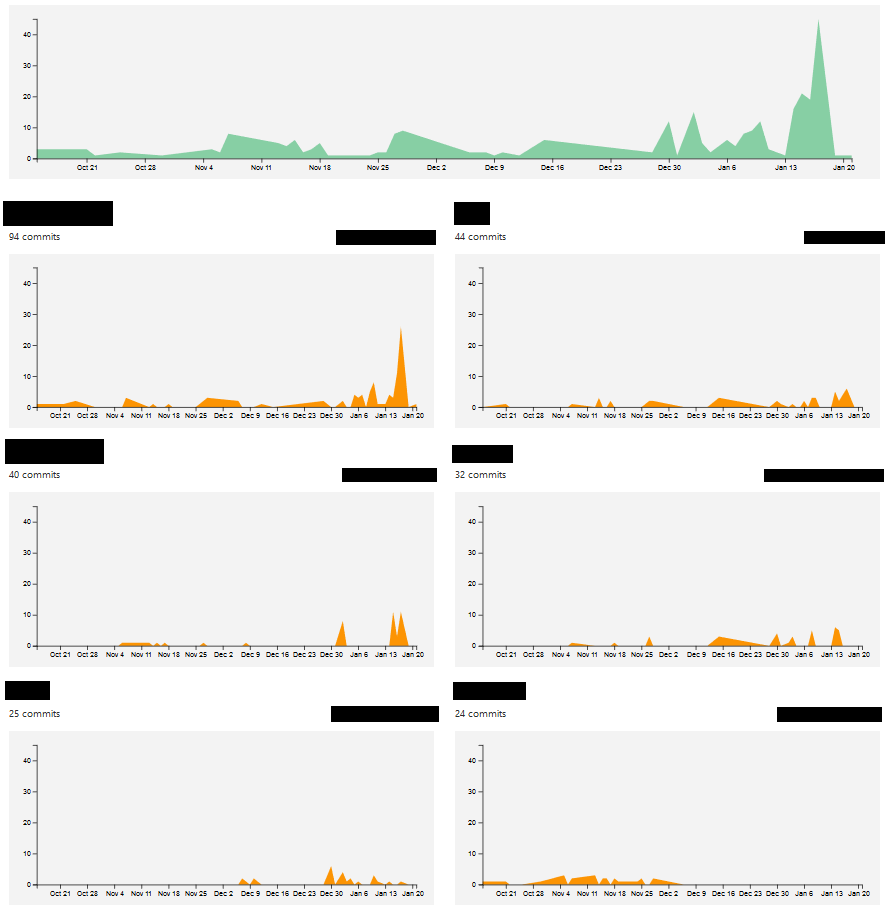
\includegraphics[scale=0.4]{slike/aktivnost.PNG} %veličina slike u odnosu na originalnu datoteku i pozicija slike
			\centering
			\caption{Primjer slike s potpisom}
			\label{fig:promjene}
		\end{figure}
		
		\begin{figure}[H]
			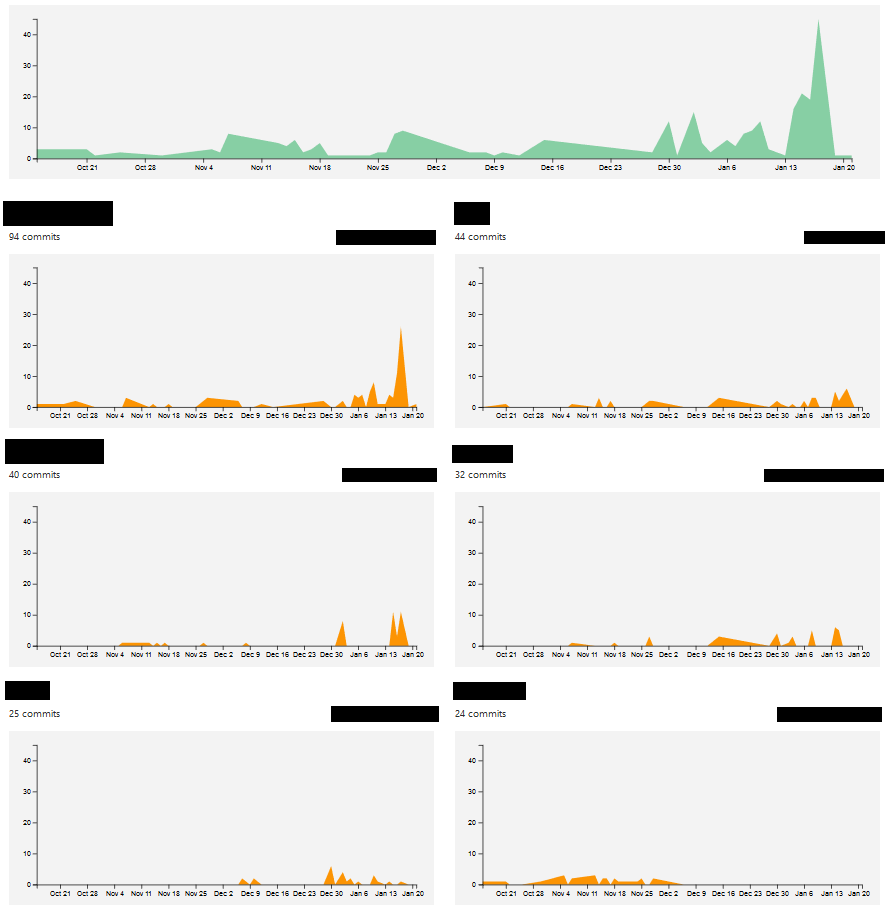
\includegraphics[width=\textwidth]{slike/aktivnost.PNG} %veličina u odnosu na širinu linije
			\caption{Primjer slike s potpisom 2}
			\label{fig:promjene2} %label mora biti drugaciji za svaku sliku
		\end{figure}
		
		Referenciranje slike \ref{fig:promjene2} u tekstu.
		
		\eject
		
	
	\chapter{Specifikacija programske potpore}
		
	\section{Funkcionalni zahtjevi}
			
			\textbf{\textit{dio 1. revizije}}\\
			
			\textit{Navesti \textbf{dionike} koji imaju \textbf{interes u ovom sustavu} ili  \textbf{su nositelji odgovornosti}. To su prije svega korisnici, ali i administratori sustava, naručitelji, razvojni tim.}\\
				
			\textit{Navesti \textbf{aktore} koji izravno \textbf{koriste} ili \textbf{komuniciraju sa sustavom}. Oni mogu imati inicijatorsku ulogu, tj. započinju određene procese u sustavu ili samo sudioničku ulogu, tj. obavljaju određeni posao. Za svakog aktora navesti funkcionalne zahtjeve koji se na njega odnose.}\\
			
			
			\noindent \textbf{Dionici:}
			
			\begin{packed_enum}
				
				\item Dionik 1
				\item Dionik 2				
				\item ...
				
			\end{packed_enum}
			
			\noindent \textbf{Aktori i njihovi funkcionalni zahtjevi:}
			
			
			\begin{packed_enum}
				\item  \underbar{Aktor 1 (inicijator) može:}
				
				\begin{packed_enum}
					
					\item funkcionalnost 1
					\item funkcionalnost 2
					\begin{packed_enum}
						
						\item  podfunkcionalnost 1 
						\item  podfunkcionalnost 2
				
					\end{packed_enum}
					\item  funkcionalnost 3
					
				\end{packed_enum}
			
				\item  \underbar{Aktor 2 (sudionik) može:}
				
				\begin{packed_enum}
					
					\item funkcionalnost 1
					\item funkcionalnost 2
					
				\end{packed_enum}
			\end{packed_enum}
			
			\eject 
			
			
				
			\subsection{Obrasci uporabe}
				
				\textbf{\textit{dio 1. revizije}}
				
				\subsubsection{Opis obrazaca uporabe}
					\textit{Funkcionalne zahtjeve razraditi u obliku obrazaca uporabe. Svaki obrazac je potrebno razraditi prema donjem predlošku. Ukoliko u nekom koraku može doći do odstupanja, potrebno je to odstupanje opisati i po mogućnosti ponuditi rješenje kojim bi se tijek obrasca vratio na osnovni tijek.}\\
					

					\noindent \underbar{\textbf{UC$<$broj obrasca$>$ -$<$ime obrasca$>$}}
					\begin{packed_item}
	
						\item \textbf{Glavni sudionik: }$<$sudionik$>$
						\item  \textbf{Cilj:} $<$cilj$>$
						\item  \textbf{Sudionici:} $<$sudionici$>$
						\item  \textbf{Preduvjet:} $<$preduvjet$>$
						\item  \textbf{Opis osnovnog tijeka:}
						
						\item[] \begin{packed_enum}
	
							\item $<$opis korak jedan$>$
							\item $<$opis korak dva$>$
							\item $<$opis korak tri$>$
							\item $<$opis korak četiri$>$
							\item $<$opis korak pet$>$
						\end{packed_enum}
						
						\item  \textbf{Opis mogućih odstupanja:}
						
						\item[] \begin{packed_item}
	
							\item[2.a] $<$opis mogućeg scenarija odstupanja u koraku 2$>$
							\item[] \begin{packed_enum}
								
								\item $<$opis rješenja mogućeg scenarija korak 1$>$
								\item $<$opis rješenja mogućeg scenarija korak 2$>$
								
							\end{packed_enum}
							\item[2.b] $<$opis mogućeg scenarija odstupanja u koraku 2$>$
							\item[3.a] $<$opis mogućeg scenarija odstupanja  u koraku 3$>$
							
						\end{packed_item}
					\end{packed_item}
				
					
				\subsubsection{Dijagrami obrazaca uporabe}
					
					\textit{Prikazati odnos aktora i obrazaca uporabe odgovarajućim UML dijagramom. Nije nužno nacrtati sve na jednom dijagramu. Modelirati po razinama apstrakcije i skupovima srodnih funkcionalnosti.}
				\eject		
				
			\subsection{Sekvencijski dijagrami}
				
				\textbf{\textit{dio 1. revizije}}\\
				
				\textit{Nacrtati sekvencijske dijagrame koji modeliraju najvažnije dijelove sustava (max. 4 dijagrama). Ukoliko postoji nedoumica oko odabira, razjasniti s asistentom. Uz svaki dijagram napisati detaljni opis dijagrama.}
				\eject
	
		\section{Ostali zahtjevi}
		
			\begin{packed_item}
				\item Cijeli sustav namijenjen je upotrebi na hrvatskom jeziku
				\item Sustav mora biti u mogućnosti podržati veći broj korisnika zbog svoje namjene
				\item Upotreba gotove aplikacije zamišljena je preko web preglednika
				\item Aplikacija mora implementirati autentikaciju i autorizaciju svakog korisnika
				\item Osjetljivi podaci od korisnika se moraju pretvarati u hash prije spremanja u bazu
				\item Greška u jednom djelu sustava ne smije onemogućiti korištenje drugih usluga
				\item Odgovori sustava prema korisniku moraju biti brzi i ne dulji od nekoliko sekundi
			\end{packed_item}
			 
			 
			 
	
	\chapter{Arhitektura i dizajn sustava}
	\textit{Arhitektura cijelog sustava može se podijeliti na četiri ključna dijela:}
		\begin{itemize}
    		\item Web preglednik
    		\item Web aplikacija
    		\item Baza podataka
    		\item Code runner
		\end{itemize}

	\textit{\underline{Web preglednik} omogućuje interakciju između korisnika i aplikacije. Svaki se korisnikov zahtjev
	 događa na web pregledniku i prosljeđuje aplikaciji na obradu. Osim slanja zahtjeva, korisniku se omogućuje
	  bolji pregled aplikacije pomoću apstraktnog koda kojeg web preglednik pretvara u lako shvatljive strukture.}\\

	\textit{\underline{Aplikacija} se sastoji od dva glavna dijela, frontenda i backenda. Tehnologije koje se koriste na backendu
	 uključuju programski jezik \textbf{Python} i \textbf{fastApi} web framework koji omogućuje stvaranje aplikacije temeljene na \textbf{REST}
	 arhitekturi i rutera na kojem su definirane rute za slanje zahtjeva i komunikaciju korisnika i aplikacije.
	 Frontend aplikacije izrađen je korištenjem JavaScript librarya \textbf{React}. On omogućuje korisniku jednostavan pregled
	 aplikacije i jednostavno korištenje aplikacije, odnosno slanje zahtjeva.}\\

	\textit{\underline{Kontejneri} se koriste unutar aplikacije kako bi poboljšali korisničko iskustvo, optimizirali performanse sustava
	te osigurali skalabilnost za povećani broj korisnika. Glavni se dio aplikacije s ruterima i logikom za komunikaciju s 
	bazom nalazi u vlastitom kontejneru kao i glavna baza, evaluator i blob storage.}\\

	\textit{Za \underline{bazu podataka} se koristi \textbf{SQL} specifično \textbf{PostgreSQL}. Glavna baza se nalazi u vlastitom kontejneru kojemu backend
	aplikacije pristupa kako bi spremio informacije u nju. Na backendu se koristi \textbf{psycopg} PostgreSQL adapter koji omogućuje
	komunikaciju između baze i backenda.}\\
	
	\textit{\underline{Evaluator} komunicira s vanjskim \underline{Code runnerom} za kompajliranje kodova koje korisnik šalje
	na backend. Ovaj ključni dio sustava odgovoran je za izvršavanje kôda unutar sigurnog okruženja, čime se osigurava
	izolacija korisničkih skripti od ostatka aplikacije. Kroz ovu komunikaciju, Evaluator prima kôd od korisnika,
	proslijeđuje ga Code runneru na izvršavanje te zatim interpretira rezultate kako bi ih pravilno integrirao
	natrag u aplikaciju.}

	\textit{Dodatno, evaluator koristi \textbf{blob storage} pomoću kojeg dohvaća podatke koji su mu potrebni za
	evaluaciju određenog zadatka. Evaluator ima pristup informacijama poput ulaznih podataka za testiranje,
	očekivanih rezultata te drugih specifičnih parametara vezanih uz pojedini zadatak.}
	
	\newpage
	
		

		

				
		\section{Baza podataka}
			
			\textbf{\textit{dio 1. revizije}}\\
			
		\textit{Potrebno je opisati koju vrstu i implementaciju baze podataka ste odabrali, glavne komponente od kojih se sastoji i slično.}
		
			\subsection{Opis tablica}
			

				\textit{Svaku tablicu je potrebno opisati po zadanom predlošku. Lijevo se nalazi točno ime varijable u bazi podataka, u sredini se nalazi tip podataka, a desno se nalazi opis varijable. Svjetlozelenom bojom označite primarni ključ. Svjetlo plavom označite strani ključ}
				
				
				\begin{longtblr}[
					label=none,
					entry=none
					]{
						width = \textwidth,
						colspec={|X[6,l]|X[6, l]|X[20, l]|}, 
						rowhead = 1,
					} %definicija širine tablice, širine stupaca, poravnanje i broja redaka naslova tablice
					\hline \SetCell[c=3]{c}{\textbf{korisnik - ime tablice}}	 \\ \hline[3pt]
					\SetCell{LightGreen}IDKorisnik & INT	&  	Lorem ipsum dolor sit amet, consectetur adipiscing elit, sed do eiusmod  	\\ \hline
					korisnickoIme	& VARCHAR &   	\\ \hline 
					email & VARCHAR &   \\ \hline 
					ime & VARCHAR	&  		\\ \hline 
					\SetCell{LightBlue} primjer	& VARCHAR &   	\\ \hline 
				\end{longtblr}
				
				
			
			\subsection{Dijagram baze podataka}
				\textit{ U ovom potpoglavlju potrebno je umetnuti dijagram baze podataka. Primarni i strani ključevi moraju biti označeni, a tablice povezane. Bazu podataka je potrebno normalizirati. Podsjetite se kolegija "Baze podataka".}
			
			\eject
			
			
		\section{Dijagram razreda}
		
			\textit{Potrebno je priložiti dijagram razreda s pripadajućim opisom. Zbog preglednosti je moguće dijagram razlomiti na više njih, ali moraju biti grupirani prema sličnim razinama apstrakcije i srodnim funkcionalnostima.}\\
			
			\textbf{\textit{dio 1. revizije}}\\
			
			\textit{Prilikom prve predaje projekta, potrebno je priložiti potpuno razrađen dijagram razreda vezan uz \textbf{generičku funkcionalnost} sustava. Ostale funkcionalnosti trebaju biti idejno razrađene u dijagramu sa sljedećim komponentama: nazivi razreda, nazivi metoda i vrste pristupa metodama (npr. javni, zaštićeni), nazivi atributa razreda, veze i odnosi između razreda.}\\
			
			\textbf{\textit{dio 2. revizije}}\\			
			
			\textit{Prilikom druge predaje projekta dijagram razreda i opisi moraju odgovarati stvarnom stanju implementacije}
			
			
			
			\eject
		
		\section{Dijagram stanja}
			
			
			\textbf{\textit{dio 2. revizije}}\\
			
			\textit{Potrebno je priložiti dijagram stanja i opisati ga. Dovoljan je jedan dijagram stanja koji prikazuje \textbf{značajan dio funkcionalnosti} sustava. Na primjer, stanja korisničkog sučelja i tijek korištenja neke ključne funkcionalnosti jesu značajan dio sustava, a registracija i prijava nisu. }
			
			
			\eject 
		
		\section{Dijagram aktivnosti}
			
			\textbf{\textit{dio 2. revizije}}\\
			
			 \textit{Potrebno je priložiti dijagram aktivnosti s pripadajućim opisom. Dijagram aktivnosti treba prikazivati značajan dio sustava.}
			
			\eject
		\section{Dijagram komponenti}
		
			\textbf{\textit{dio 2. revizije}}\\
		
			 \textit{Potrebno je priložiti dijagram komponenti s pripadajućim opisom. Dijagram komponenti treba prikazivati strukturu cijele aplikacije.}
	\chapter{Implementacija i korisničko sučelje}
		
		
		\section{Korištene tehnologije i alati}
		
			Komunikacija u timu ostvarena je kombinacijom \textbf{Atlassin Jira}, \textbf{Atlassin Confluence} i \textbf{WhatsApp}. Za upravljanje kodom korišten je sustav \textbf{Git} i web platforma \textbf{GitHub} za pregled udaljenog repozitorija i bolje snalaženje u projektu.
			Kao razvojno okruženje korišteni su \textbf{Microsoft Visual Studio Code} i \textbf{JetBrains PyCharm}. Microsoft Visual Studio Code pruža integrirano razvojno okruženje (IDE) koje podržava različite programske jezike, uključujući C++, Python i mnoge druge. Ovo okruženje dolazi s alatima za uređivanje koda, debugiranje i upravljanje datotekama i kontejnerima.
			S druge strane, \textbf{JetBrains PyCharm} je posebno usmjeren na podršku Python razvoju. Ovaj IDE pruža bogat skup značajki, uključujući pametno završavanje koda, analizu koda, integrirano upravljanje verzijama, i podršku za virtualno okruženje. Korištenjem ova dva razvojna okruženja, tim je imao pristup snažnim alatima za učinkovit i produktivan razvoj softvera.
			Aplikacija je napisana koristeći radni okvir \textbf{FastApi} koji se koristi za izradu REST API-ja u pythonu. Za izradu \textit{frontenda} koristili smo \textbf{React} i \textbf{TypeScript}. Prednost \textbf{TypeScripta} nad običnim \textbf{Javascriptom} je u njegovoj mogućnosti definiranja tipa varijabli i posljedično tome, lakšem rukovanju greškama i boljom kontrolom varijabli.
			Za izradu kontejnera je korišten \textbf{Docker}, a sve je stavljeno na poslužitelja u oblaku na \textbf{Microsoft Azure}.
			
			
			
			\eject 
		
	
		\section{Ispitivanje programskog rješenja}
			
			
			\subsection{Ispitivanje komponenti}
			
			\subsubsection{Ispitni slučaj 1: Registracija korisnika}
				\begin{packed_item}
					
					\item Testira se rad funkcije \texttt{register()} iz \texttt{auth\_services.py}.
					\item Mock-anje autentikacije i spremanja korisnika u bazu.
					\item Očekivani response: HTTP 201 CREATED.
				\end{packed_item}
				
			\subsubsection{Ispitni slučaj 2: Prijava korisnika}
				\begin{packed_item}
					\item Testira se funkcija login() za ulogiravanje postojećeg korisnika uz mockanje tokena
					\item Očekivani response: HTTP 200
				\end{packed_item}
			
			\subsubsection{Ispitni slučaj 3: Ispravno kreiranje problema}
				\begin{packed_item}
					\item Testira se funkcija \texttt{create\_problem()}
					\item Mock-anje form date za popunjavanje forme za kreiranje problema.
					\item Očekivani response: HTTP 201 CREATED
				\end{packed_item}
			
			\subsubsection{Ispitni slučaj 4: Neispravno kreiranje problema}
				\begin{packed_item}
					\item Form data popunjena neispravnim podacima.
					\item očekivani response: HTTP 422
			 	\end{packed_item}	
			 	
			\subsubsection{Ispitni slučaj 5: Ispravno kreiranje natjecanja}
				\begin{packed_item}
					\item Mock- anje form date za kreiranje natjecanja
					\item Očekivani response: HTTP 201 CREATED
				\end{packed_item}
				
			\subsubsection{Ispitni slučaj 6: Neispravno kreiranje natjecanja}
				\begin{packed_item}
					\item Mock form date s nedovoljno podataka
					\item Očekivani response: HTTP 422
				\end{packed_item}
				
			\eject
			
			
			\subsection{Ispitivanje sustava}
			
			\subsubsection{Ispitni slučaj 1: Ispravna prijava u sustav}
			
			
			\noindent {\textbf{Ulaz:}}
			\begin{packed_enum}
				
				\item  Otvaranje početne stranice u web pregledniku.
				\item  Pritisak na gumb \textbf{Login} u gornjem desnom kutu.
				\item  Ispravno ispunjavanje forme za prijavu.
				\item  Pritisak na gumb \textbf{Submit}. 
				
			\end{packed_enum}
			
			\noindent {\textbf{Očekivani rezultat:}}
			\begin{packed_enum}
				
				\item  Prikaz početne stranice korisnika. 
				
			\end{packed_enum}
			
			\noindent \textbf{Rezultat:} Očekivani rezultat [1.] je zadovoljen jer je korisnik ispravno unio podatke. \textbf{Aplikacija je prošla test.}
			
			\begin{figure}[H]
				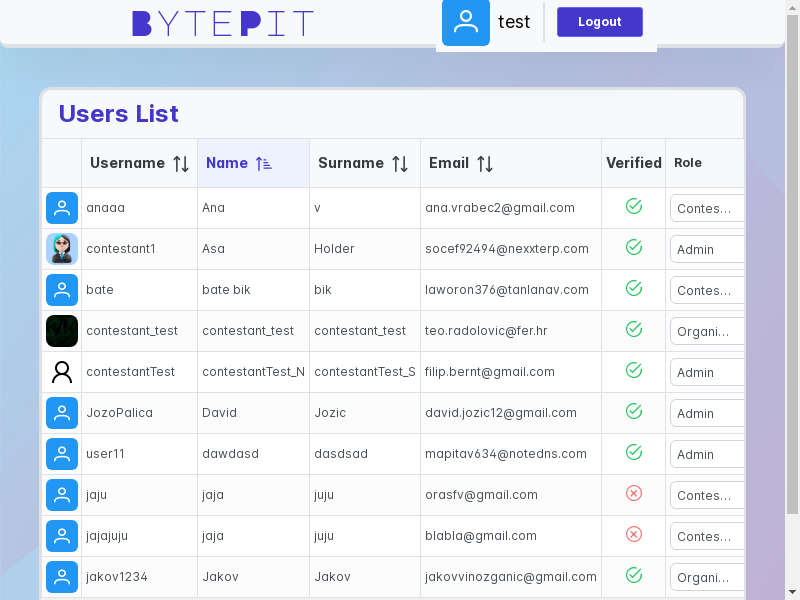
\includegraphics[scale=0.50]{slike/screenshot_test_result.PNG}
				\centering
				\caption{Uspješna prijava}
				\label{fig:sucess_login}
			\end{figure}
			
			\eject
			
			\subsubsection{Ispitni slučaj 2: Neispravna prijava u sustav}
			
			
			\noindent {\textbf{Ulaz:}}
			\begin{packed_enum}
				
				\item  Otvaranje početne stranice u web pregledniku.
				\item  Pritisak na gumb \textbf{Login} u gornjem desnom kutu.
				\item  Ispunjavanje forme za prijavu.
				\item  Pritisak na gumb \textbf{Submit}. 
				
			\end{packed_enum}
			
			\noindent {\textbf{Očekivani rezultat:}}
			\begin{packed_enum}
				
				\item  Prikaz oblačića sa tekstom koji govori da je pogrešno unesena zaporka ili e-pošta/korisničko ime. 
				
			\end{packed_enum}
			
			\noindent \textbf{Rezultat:} Očekivani rezultat [1.] je zadovoljen jer je korisnik unio pogrešnu zaporku. \textbf{Aplikacija je prošla test.}
			
			\begin{figure}[H]
				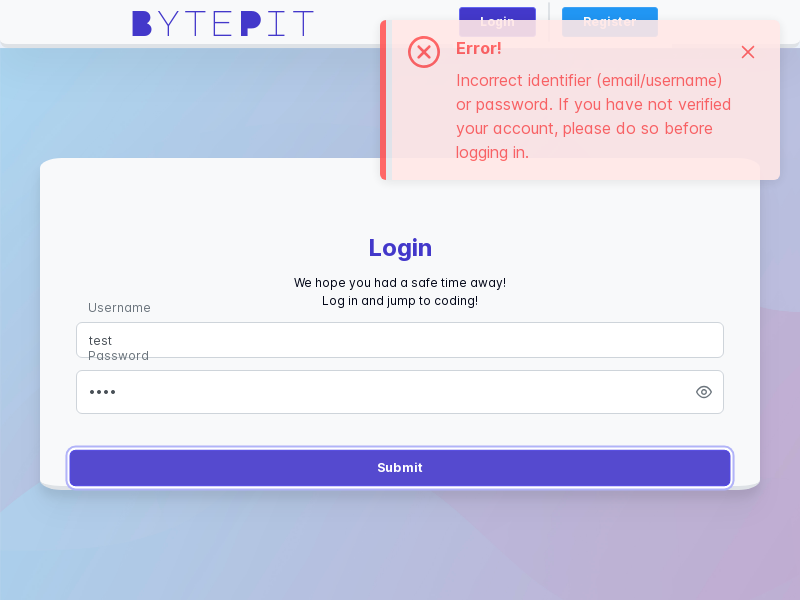
\includegraphics[scale=0.50]{slike/failed_login.PNG}
				\centering
				\caption{Neuspješna prijava}
				\label{fig:failed_login}
			\end{figure}
			
			\eject
			
			\subsubsection{Ispitni slučaj 3: Ispravna registracija novog korisnika}
			
			
			\noindent {\textbf{Ulaz:}}
			\begin{packed_enum}
				
				\item  Otvaranje početne stranice u web pregledniku.
				\item  Pritisak na gumb \textbf{Register} u gornjem desnom kutu.
				\item  Ispunjavanje forme za registraciju.
				\item  Pritisak na gumb \textbf{Submit}. 
				
			\end{packed_enum}
			
			\noindent {\textbf{Očekivani rezultat:}}
			\begin{packed_enum}
				
				\item  Uspješno slanje forme za kreaciju novog korisnika.
				\item  Dobitak e-pošte za verifikaciju novog računa.
				
			\end{packed_enum}
			
			\noindent \textbf{Rezultat:} Očekivani rezultati [1., 2.] su zadovoljeni jer je korisnik ispravno unio podatke koji su traženi. \textbf{Aplikacija je prošla test.}
			
			\begin{figure}[H]
				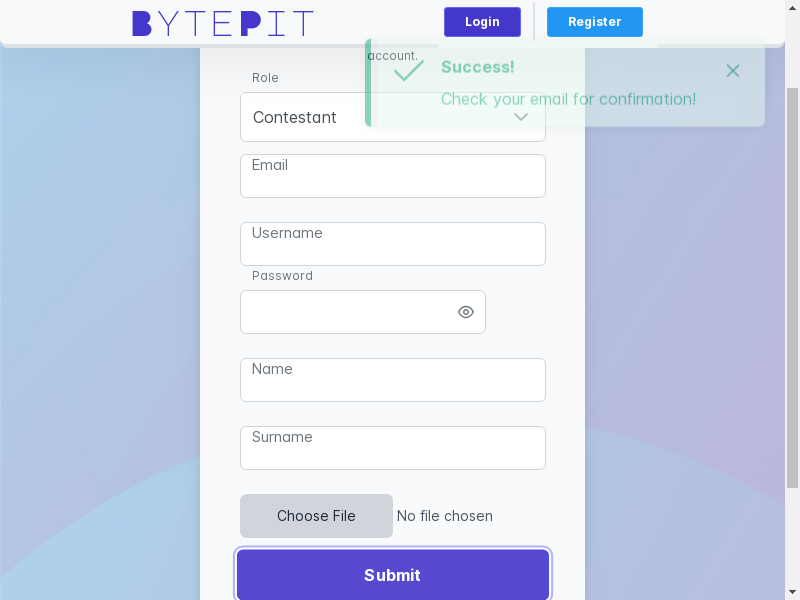
\includegraphics[scale=0.50]{slike/registration_new_user_test_result.PNG}
				\centering
				\caption{Uspješna registracija}
				\label{fig:sucess_register}
			\end{figure}
			
			\eject
			
			\subsubsection{Ispitni slučaj 4: Neispravna registracija novog korisnika}
			
			
			\noindent {\textbf{Ulaz:}}
			\begin{packed_enum}
				
				\item  Otvaranje početne stranice u web pregledniku.
				\item  Pritisak na gumb \textbf{Register} u gornjem desnom kutu.
				\item  Neispravno ispunjavanje forme za registraciju (korištenje e-pošte koja se već nalazi u sustavu).
				\item  Pritisak na gumb \textbf{Submit}. 
				
			\end{packed_enum}
			
			\noindent {\textbf{Očekivani rezultat:}}
			\begin{packed_enum}
				
				\item  Neuspješno slanje forme za kreaciju novog korisnika.
				\item  Prikaz oblačića sa tekstom koji govori da se e-pošta već koristi.
				
			\end{packed_enum}
			
			\noindent \textbf{Rezultat:} Očekivani rezultati [1., 2.] su zadovoljeni jer je korisnik unio e-poštu koja se već koristi. \textbf{Aplikacija je prošla test.}
			
			\begin{figure}[H]
				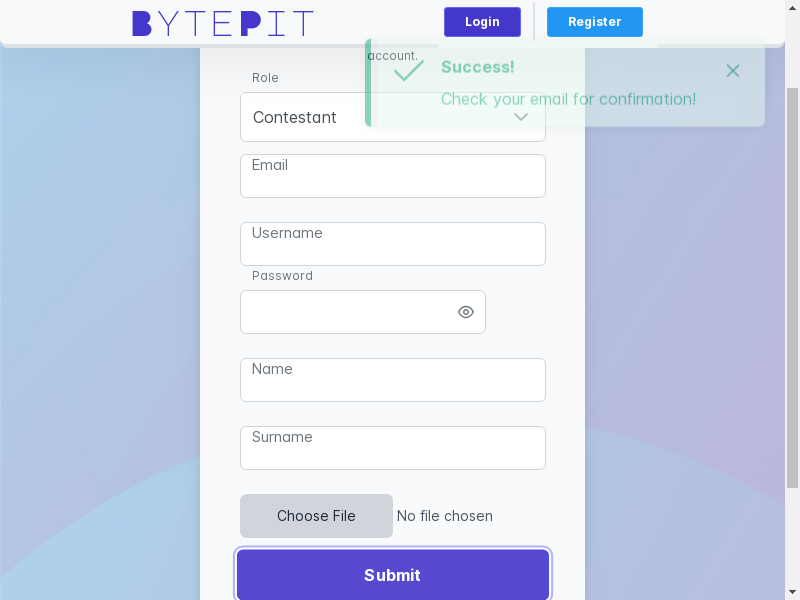
\includegraphics[scale=0.50]{slike/registration_new_user_test_result.PNG}
				\centering
				\caption{Uspješna registracija}
				\label{fig:failed_register}
			\end{figure}
			
			\eject
			
			\subsubsection{Ispitni slučaj 5: Uspješno kreiranje zadatka}
			
			
			\noindent {\textbf{Ulaz:}}
			\begin{packed_enum}
				
				\item  Prikaz početne stranice voditelja (samo voditelj ima opciju kreacije zadatka).
				\item  Pritisak na gumb \textbf{New Problem}.
				\item  Prikaz forme za kreaciju problema.
				\item  Ispravno ispunjavanje forme za kreaciju zadatka.
				
			\end{packed_enum}
			
			\noindent {\textbf{Očekivani rezultat:}}
			\begin{packed_enum}
				
				\item  Uspješna kreacija novog zadatka.
				
			\end{packed_enum}
			
			\noindent \textbf{Rezultat:} Očekivani rezultat [1.] je zadovoljen jer je korisnik ispravno ispunio formu za izradu novog zadatka. \textbf{Aplikacija je prošla test.}
			
			\begin{figure}[H]
				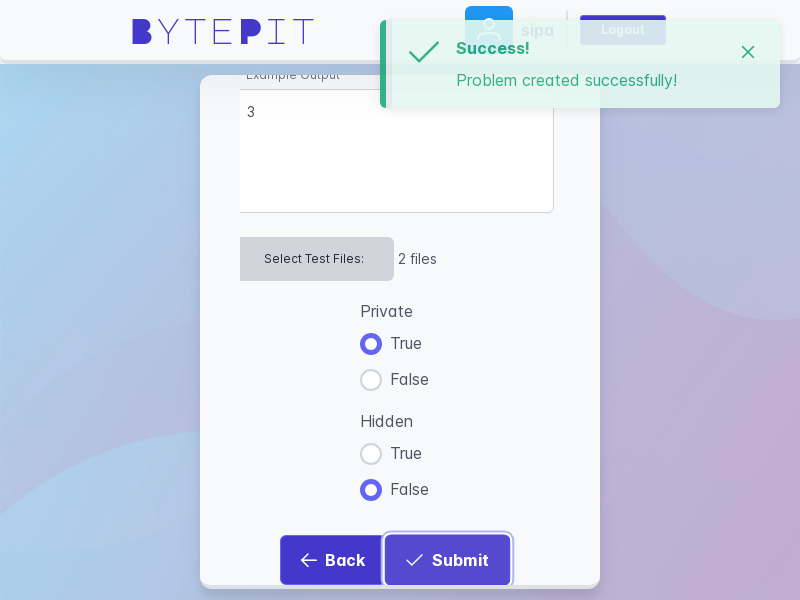
\includegraphics[scale=0.50]{slike/create_problem_test.PNG}
				\centering
				\caption{Uspješna izrada novog zadatka}
				\label{fig:sucess_new_problem}
			\end{figure}
			
			\eject
			
			\subsubsection{Ispitni slučaj 6: Neuspješno kreiranje zadatka}
			
			
			\noindent {\textbf{Ulaz:}}
			\begin{packed_enum}
				
				\item  Prikaz početne stranice voditelja (samo voditelj ima opciju kreacije zadatka).
				\item  Pritisak na gumb \textbf{New Problem}.
				\item  Prikaz forme za kreaciju problema.
				\item  Neispravno ispunjavanje forme za kreaciju zadatka (broj bodova zadatka ne smije biti nula).
				
			\end{packed_enum}
			
			\noindent {\textbf{Očekivani rezultat:}}
			\begin{packed_enum}
				
				\item  Prikaz oblačića sa tekstom koji govori da broj bodova zadatka ne smije biti jednak nuli.
				
			\end{packed_enum}
			
			\noindent \textbf{Rezultat:} Očekivani rezultat [1.] je zadovoljen jer je korisnik neispravno ispunio formu za izradu novog zadatka. \textbf{Aplikacija je prošla test.}
			
			\begin{figure}[H]
				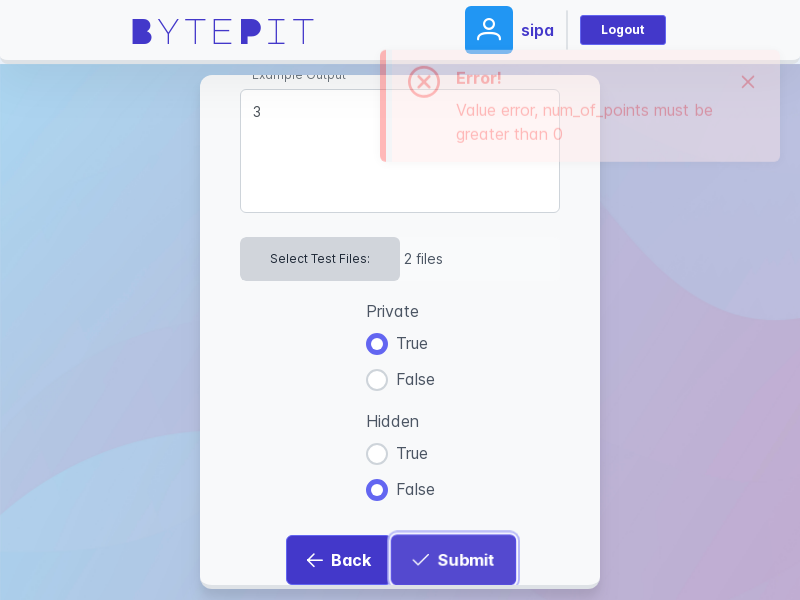
\includegraphics[scale=0.50]{slike/create_problem_test_wrong.PNG}
				\centering
				\caption{Neuspješna izrada novog zadatka}
				\label{fig:failed_new_problem}
			\end{figure}
			
			\eject
			
			\subsubsection{Ispitni slučaj 7: Uspješna odjava korisnika}
			
			
			\noindent {\textbf{Ulaz:}}
			\begin{packed_enum}
				
				\item  Pritisak na gumb \textbf{Logout} na stranici korisnika.
				
			\end{packed_enum}
			
			\noindent {\textbf{Očekivani rezultat:}}
			\begin{packed_enum}
				
				\item  Prikaz stranice za prijavu u sustav.
				
			\end{packed_enum}
			
			\noindent \textbf{Rezultat:} Očekivani rezultat [1.] je zadovoljen. \textbf{Aplikacija je prošla test.}
			
			\begin{figure}[H]
				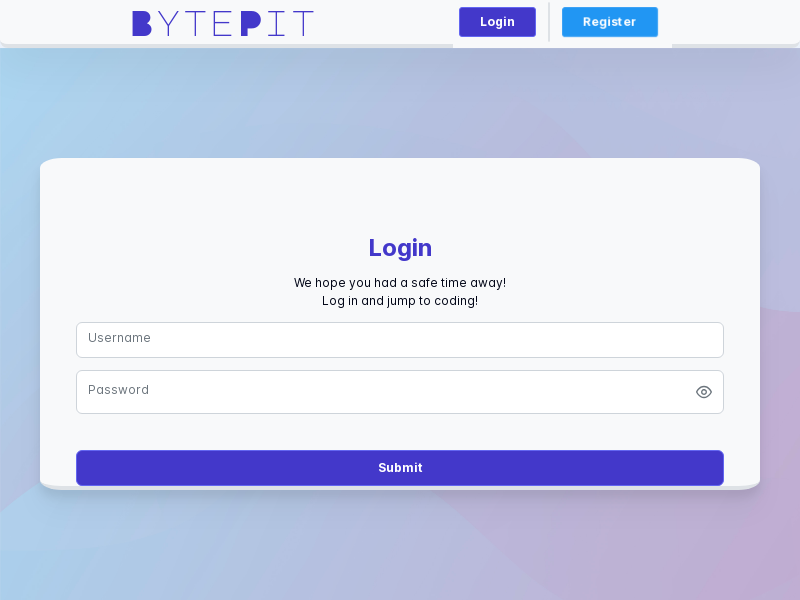
\includegraphics[scale=0.50]{slike/screen_after_logout.PNG}
				\centering
				\caption{Uspješna odjava}
				\label{fig:sucess_logout}
			\end{figure}
			
			
			\eject 
		
		
		\section{Dijagram razmještaja}

			 Dijagrami razmještaja opisuju topologiju sklopovlja i programsku potporu koja se koristi u implementaciji sustava u njegovom radnom okruženju.
			 Na azure app service-u nalaze se API sa evaluatorom rješenja, poslužitelj baze podataka (azure sql database) te third party servis za kompajliranje koda.
			 Klijenti koriste web preglednik za pristup web aplikaciji. Sustav je baziran na REST API arhitekturi, a komunikacija između klijenta i poslužitelja odvija se preko HTTP veze.

			 
			
			\begin{figure}[H]
				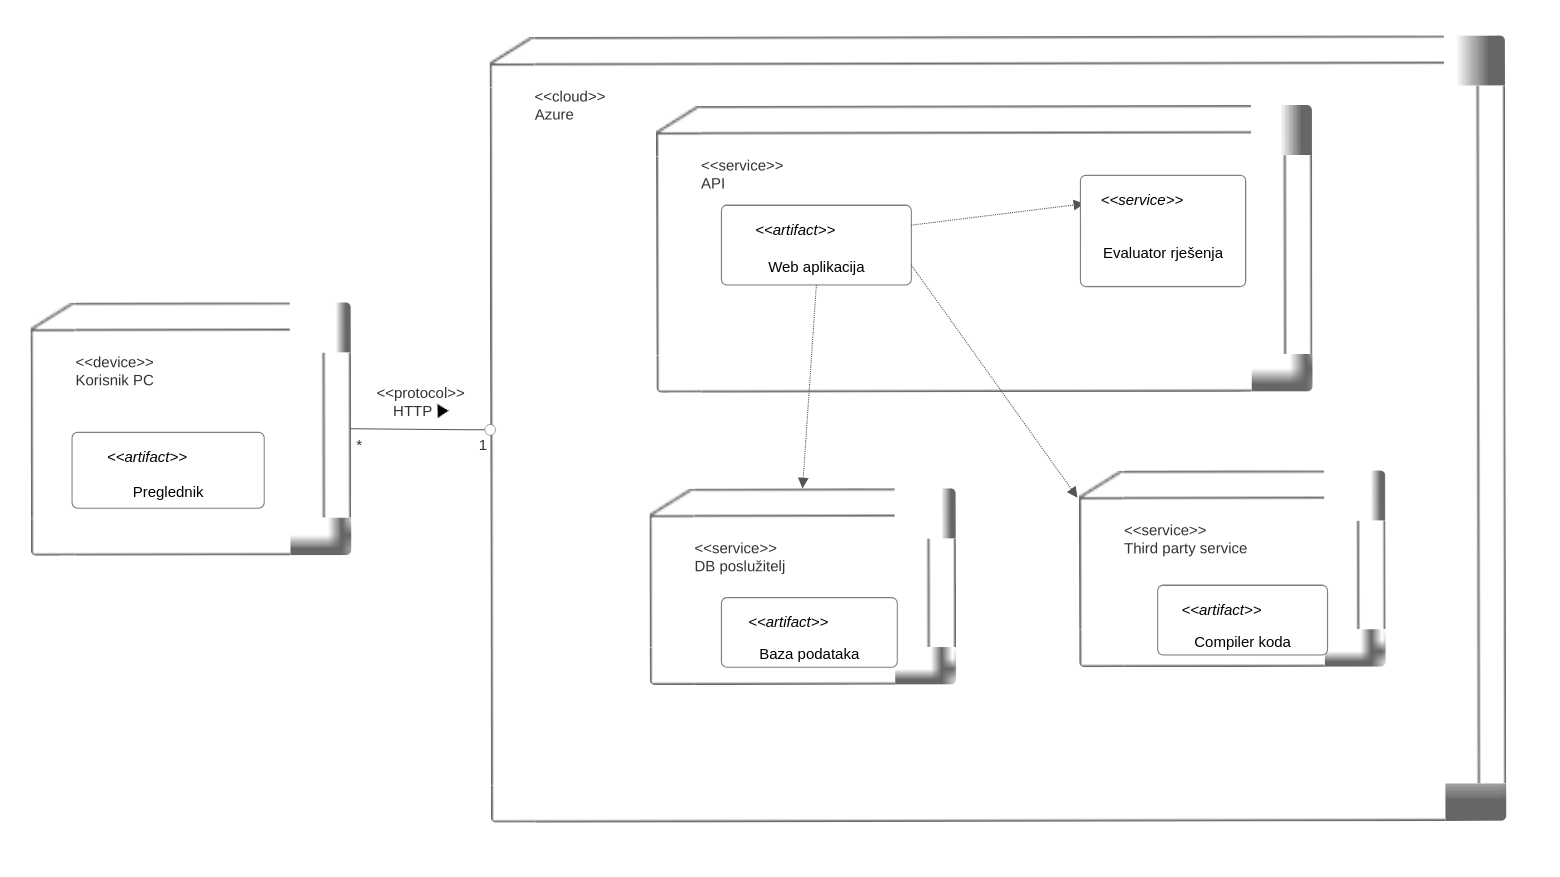
\includegraphics[width=\linewidth]{slike/dijagram_razmjestaja.png} 
				\centering
				\caption{Dijagram razmještaja}
				\label{fig:razmjestaj}
			\end{figure}
			\eject 
		
		\section{Upute za puštanje u pogon}
		
			\textbf{Pokretanje backend-a i baze podataka}\\
			
				\noindent Potrebno je preuzeti i instalirati aplikaciju \href{https://www.docker.com/products/docker-desktop/}{Docker Desktop} uz pomoć koje se pokreću container-i za backend i bazu podataka. Nakon preuzimanja aplikacije moramo se u terminalu navigirati do direktorija \textit{bytepit-root} unutar kojeg se nalazi docker-compose datoteka koja sadrži informacije za pokretanje. Pri prvom pokretanju potrebno je nekoliko minuta za podizanje.\\
				Unutar terminala koristimo naredbu: \textbf{docker-compose up --build}
				\begin{figure}[H]
					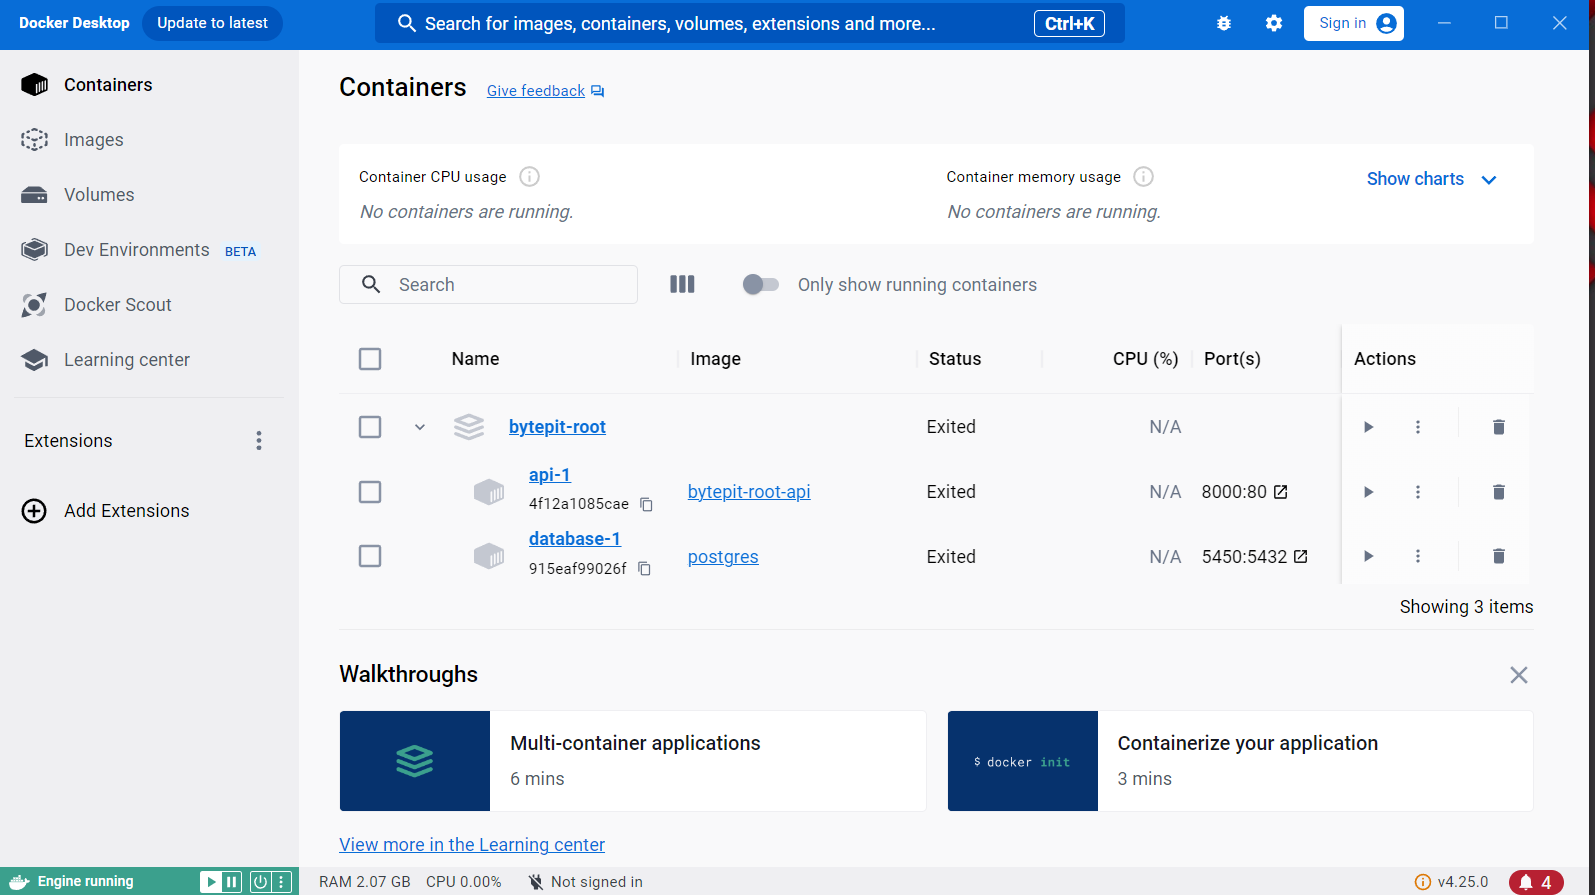
\includegraphics[scale=0.45]{slike/docker_desktop.PNG} 
					\centering
					\caption{Aplikacija Docker Desktop sa kreiranim containerima}
					\label{fig:docker_desktop}
				\end{figure}
				\noindent Pri prvom pokretanju unutar baze neće biti kreirane potrebne tablice, ali ih možemo kreirati uz pomoć datoteke \textbf{ddl.sql} koja se nalazi unutar direktorija \textit{bytepit-root}. Unutar aplikacije Docker Desktop možemo kliknuti na opcije od baze (tri uspravne točkice ispod zaglavlja Actions), te odabrati opciju \textbf{Open in terminal} uz pomoć koje možemo upisati naredbe za kreaciju tablica unutar baze. Unutar terminala odabiremo opciju \textbf{Exec} te u njoj napišemo naredbu: \textbf{psql -U postgres -d db}\\
				\eject
				\noindent Tada možemo pisati naredbe za našu bazu u SQL-u unutar terminala. Sljedeća naredba koju unosimo je cijela \textbf{ddl.sql} datoteka uz pomoć koje se kreiraju tablice. Nakon toga su backend i baza podataka uspješno postavljeni i spremni za korištenje. Kao provjeru za ispravno kreiranje tablica možemo napisati query poput ovoga:\\
				\textbf{SELECT * FROM problems;}, u slučaju ispravnog postavljanja ispisuje se tablica \textit{problems}.\\
				\begin{figure}[H]
					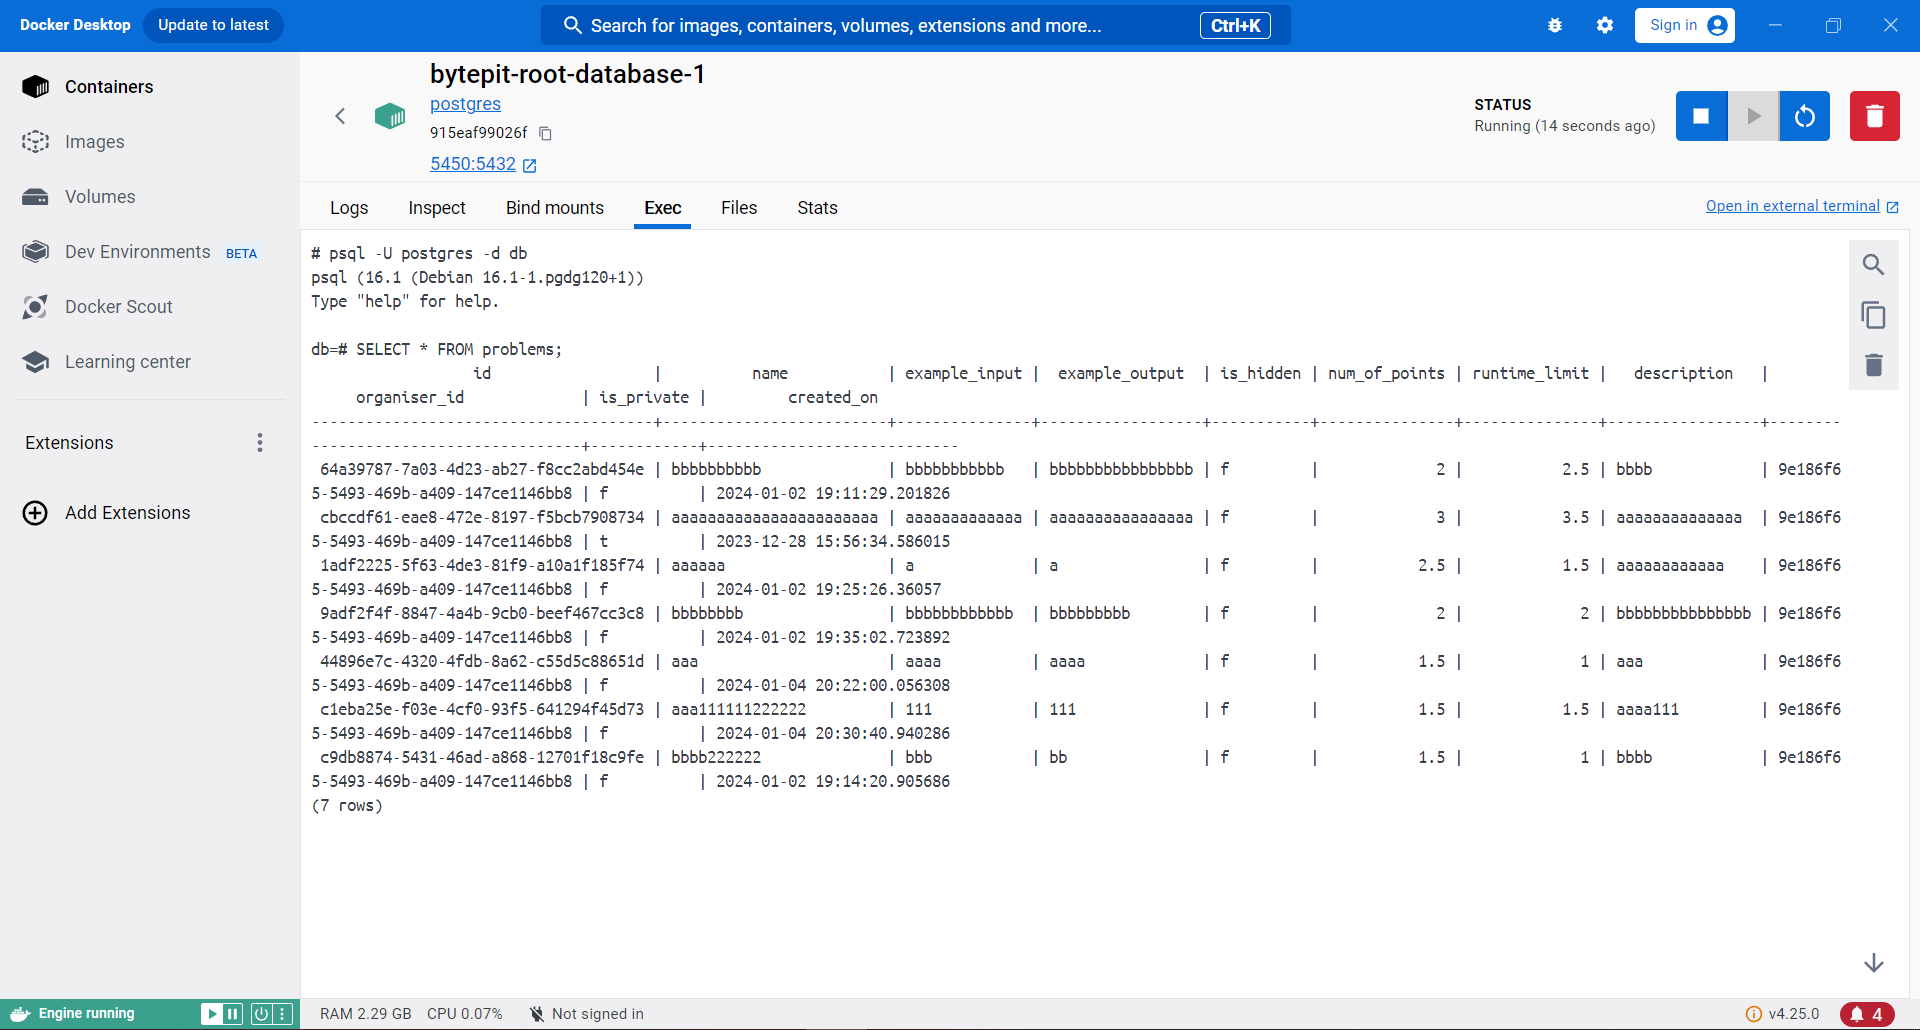
\includegraphics[scale=0.4]{slike/postgres.PNG} 
					\centering
					\caption{Ispravno ispunjena baza i provjera}
					\label{fig:docker_desktop_postgres}
				\end{figure}
				\noindent Za zaustavljanje Docker container-a koristimo naredbu: \textbf{docker-compose down}\\
				
			\eject
			
			\noindent\textbf{Pokretanje frontend-a}\\
			
			\noindent Unutar terminala se navigiramo do direktorija \textit{bytepit-ui} te pokrećemo naredbu: \textbf{npm install}\\
			Pomoću te naredbe se pokreće instalacija Vite-a i ostalih dependency-a koji su potrebni za pokretanje frontend-a. Za instalaciju je potrebno nekoliko minuta.\\
			\noindent Nakon instalacije pokrećemo naredbu: \textbf{npm run dev} koja pokreće frontend.
			\begin{figure}[H]
				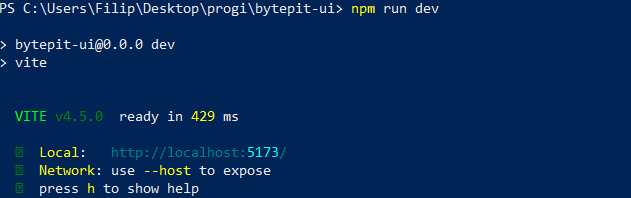
\includegraphics[scale=0.9]{slike/vite.PNG} 
				\centering
				\caption{Terminal nakon uspješno izvedene funkcije za pokretanje}
				\label{fig:vite}
			\end{figure}
			\noindent Tada možemo otvoriti web-preglednik i upisati \textbf{http://localhost:5173/} i početi koristiti aplikaciju.\\
			\begin{figure}[H]
				
\includegraphics[scale=0.4]{slike/bytepit.PNG} 
				\centering
				\caption{Pokrenuta aplikacija}
				\label{fig:bytepit}
			\end{figure}
			Za zaustavljanje koristimo naredbu: \textbf{npm run stop}\\
			
	\chapter{Zaključak i budući rad}
		
		\textbf{\textit{dio 2. revizije}}\\
		
		 \textit{U ovom poglavlju potrebno je napisati osvrt na vrijeme izrade projektnog zadatka, koji su tehnički izazovi prepoznati, jesu li riješeni ili kako bi mogli biti riješeni, koja su znanja stečena pri izradi projekta, koja bi znanja bila posebno potrebna za brže i kvalitetnije ostvarenje projekta i koje bi bile perspektive za nastavak rada u projektnoj grupi.}
		
		 \textit{Potrebno je točno popisati funkcionalnosti koje nisu implementirane u ostvarenoj aplikaciji.}
		
		\eject 
	\chapter*{Popis literature}
		\addcontentsline{toc}{chapter}{Popis literature}
		
		
		\begin{enumerate}
			
			
			\item  Programsko inženjerstvo, FER ZEMRIS, \url{http://www.fer.hr/predmet/proinz}
			
			\item  The Unified Modeling Language, \url{https://www.uml-diagrams.org/}
			
			\item  Astah Community, \url{http://astah.net/editions/uml-new}
			
			\item  Docker Desktop, \url{https://www.docker.com/products/docker-desktop/}
			
			\item  Primereact, \url{https://primereact.org/}
			
			\item  JSON Web tokens, \url{https://auth0.com/docs/secure/tokens/json-web-tokens}
			
			\item  CodeX-API, \url{https://github.com/Jaagrav/CodeX-API/tree/master}
			
			\item  FastAPI, \url{https://fastapi.tiangolo.com/tutorial/first-steps/}
			
			\item SQLAlchemy, \url{https://www.sqlalchemy.org/}
			
			\item Pydantic, \url{https://docs.pydantic.dev/latest/concepts/models/}
			
			\item PostgreSQL, \url{https://www.postgresql.org/}
			
			\item Vite, \url{https://vitejs.dev/}
		\end{enumerate}
		
		 
	
	
	\begingroup
	\renewcommand*\listfigurename{Indeks slika i dijagrama}
	%\renewcommand*\listtablename{Indeks tablica}
	%\let\clearpage\relax
	\listoffigures
	%\vspace{10mm}
	%\listoftables
	\endgroup
	\addcontentsline{toc}{chapter}{Indeks slika i dijagrama}


	
	\eject 
		
	\chapter*{Dodatak: Prikaz aktivnosti grupe}
		\addcontentsline{toc}{chapter}{Dodatak: Prikaz aktivnosti grupe}
		
		\section*{Dnevnik sastajanja}
		
		
		\begin{packed_enum}
			\item  sastanak
			
			\item[] \begin{packed_item}
				\item Datum: 20. listopada 2023.
				\item Prisustvovali: F.Sipić, T.Radolović, J.Franjković, J.Vinožganić, T.Matošević, F.Bernt, M.Bolt
				\item Teme sastanka:
				\begin{packed_item}
					\item  inicijalni dogovor o temi projekta
					\item  prijedlozi tehnologija i arhitekture
				\end{packed_item}
			\end{packed_item}
			
			\item  sastanak
			\item[] \begin{packed_item}
				\item Datum: 2. studenoga 2023.
				\item Prisustvovali: F.Sipić, T.Radolović, J.Franjković, J.Vinožganić, T.Matošević, F.Bernt, M.Bolt
				\item Teme sastanka:
				\begin{packed_item}
					\item  podjela u podtimove, frontend, backend, dokumentacija
				\end{packed_item}
			\end{packed_item}

			\item  sastanak
			\item[] \begin{packed_item}
				\item Datum: 4. studenoga 2023.
				\item Prisustvovali: F.Sipić, T.Radolović, J.Franjković, J.Vinožganić, T.Matošević, F.Bernt, M.Bolt
				\item Teme sastanka:
				\begin{packed_item}
					\item  dogovor o strukturi baze podataka
				\end{packed_item}
			\end{packed_item}

			\item  sastanak
			\item[] \begin{packed_item}
				\item Datum: 6. studenoga 2023.
				\item Prisustvovali: F.Sipić, T.Radolović, J.Franjković, J.Vinožganić, T.Matošević, F.Bernt, M.Bolt
				\item Teme sastanka:
				\begin{packed_item}
					\item  podjela zadataka za sljedeći tjedan
				\end{packed_item}
			\end{packed_item}

			\item  sastanak
			\item[] \begin{packed_item}
				\item Datum: 8. studenoga 2023.
				\item Prisustvovali: F.Sipić, J.Franjković, J.Vinožganić, M.Bolt
				\item Teme sastanka:
				\begin{packed_item}
					\item  dogovor o postavljanju backend okruženja
				\end{packed_item}
			\end{packed_item}

			\item  sastanak
			\item[] \begin{packed_item}
				\item Datum: 9. studenoga 2023.
				\item Prisustvovali: F.Bernt, T.Radolović, T.Matošević, M.Bolt
				\item Teme sastanka:
				\begin{packed_item}
					\item  dogovor o postavljanju frontend okruženja
				\end{packed_item}
			\end{packed_item}

			\item  sastanak
			\item[] \begin{packed_item}
				\item Datum: 14. studenoga 2023.
				\item Prisustvovali: F.Sipić, J.Franjković, J.Vinožganić, M.Bolt, T.Radolović, T.Matošević, F.Bernt
				\item Teme sastanka:
				\begin{packed_item}
					\item  dogovor o deploymentu aplikacije
				\end{packed_item}
			\end{packed_item}

			\item  sastanak
			\item[] \begin{packed_item}
				\item Datum: 5. prosinca 2023.
				\item Prisustvovali: F.Sipić, J.Franjković, J.Vinožganić, M.Bolt, T.Radolović, T.Matošević, F.Bernt
				\item Teme sastanka:
				\begin{packed_item}
					\item  dogovor o nastavku razvoja aplikacije
					\item podjela zadataka za sljedećih nekoliko tjedana
				\end{packed_item}
			\end{packed_item}

			\item  sastanak
			\item[] \begin{packed_item}
				\item Datum: 20. prosinca 2023.
				\item Prisustvovali: F.Sipić, J.Franjković, F.Bernt
				\item Teme sastanka:
				\begin{packed_item}
					\item  pregled i ispravljanje grešaka u dokumentaciji
				\end{packed_item}
			\end{packed_item}
			
			\item  sastanak
			\item[] \begin{packed_item}
				\item Datum: 14. siječnja 2024.
				\item Prisustvovali: F.Sipić, J.Franjković, F.Bernt, J. Vinožganić, T. Radolović, T. Matošević, M. Bolt
				\item Teme sastanka:
				\begin{packed_item}
					\item  finalni sastanak za završnu predaju, ispravke dokumentacije i koda
				\end{packed_item}
			\end{packed_item}
			
			%
			
		\end{packed_enum}
		
		\eject
		\section*{Tablica aktivnosti}

			\begin{longtblr}[
					label=none,
				]{
					vlines,hlines,
					width = \textwidth,
					colspec={X[7, l]X[1, c]X[1, c]X[1, c]X[1, c]X[1, c]X[1, c]X[1, c]}, 
					vline{1} = {1}{text=\clap{}},
					hline{1} = {1}{text=\clap{}},
					rowhead = 1,
				} 
			
				\SetCell[c=1]{c}{} & \SetCell[c=1]{c}{\rotatebox{90}{\textbf{Marko Bolt}}} & \SetCell[c=1]{c}{\rotatebox{90}{\textbf{Filip Bernt }}} &	\SetCell[c=1]{c}{\rotatebox{90}{\textbf{Teo Matošević }}} & \SetCell[c=1]{c}{\rotatebox{90}{\textbf{Teo Radolović }}} &	\SetCell[c=1]{c}{\rotatebox{90}{\textbf{Jure Franjković }}} & \SetCell[c=1]{c}{\rotatebox{90}{\textbf{Fran Sipić }}} &	\SetCell[c=1]{c}{\rotatebox{90}{\textbf{Jakov Vinožganić }}} \\  
				Upravljanje projektom 		& 15 &  & 4 &  &  &  & 3 \\ 
				Opis projektnog zadatka 	& 3 &  &  &  &  &  & \\ 
				
				Funkcionalni zahtjevi       &  &  &  & 3 &  & 2  & 4 \\ 
				Opis pojedinih obrazaca 	&  & 4 &  &  &  &  &  \\ 
				Dijagram obrazaca 			&  & 7 &  &  &  &  &  \\
				Sekvencijski dijagrami 		&  &  & 1 &  &  & 6 &  \\ 
				Opis ostalih zahtjeva 		&  &  &  &  & 3 &  &  \\ 

				Arhitektura i dizajn sustava	 &  &  &  &  & 3 &  &  \\ 
				Baza podataka				&  & 1 &  &  &  & 4 &   \\ 
				Dijagram razreda 			&  &  &  &  & 6 &  &   \\ 
				Dijagram stanja				&  &  &  &  &  &  3  \\ 
				Dijagram aktivnosti 		&  &  &  &  & 3 &  &  \\ 
				Dijagram komponenti			&  & 4 &  &  &  &  &  \\ 
				Korištene tehnologije i alati 		&  &  &  &  & 1 &  &  \\ 
				Ispitivanje programskog rješenja 	& 2 & 3 &  &  & 3 & 6 &  \\ 
				Dijagram razmještaja			&  &  &  &  &  & 3 &  \\ 

				Upute za puštanje u pogon 		&  & 2 &  &  &  &  &  \\  
				Dnevnik sastajanja 			&  &  &  &  &  & 1 &  \\ 

				Zaključak i budući rad 		& 2 &  &  &  &  &  &  \\  
				Popis literature 			&  & 1 &  &  &  &  &  \\   
				\textit{front end} 				& 30 & 27 & 28 & 32 & 17 & 11 & 35 \\  
				\textit{izrada baze podataka} 		 			& 2  &  & 3 &  &  &  & 4\\  
				\textit{spajanje s bazom podataka} 							& 2 &  &  &  &  &  & 2 \\ 
				\textit{back end} 							& 24 &  & 12 & 10 & 15 & 7 & 30 \\ 
				\textit{deploy} 							& 10 &  & 5 & 7 &  &  &  \\ 
				\textit{ostale stavke} 							& 8 & 15 & 11 & 10 & 12 & 7 & 9 \\ 						 
			\end{longtblr}
					
					
		\eject
		\section*{Dijagrami pregleda promjena}
		
		\noindent Na prikazanim grafovima se nalaze samo promjene grane development na svim repozitorijima, te neki članovi nisu imali podudarajuće e-mailove na lokalnom računalu i GitHub-u zato se ne prikazuju kao \textit{Contributors}. Također se ne prikazuje aktivnost na svim granama već samo na development jer GitHub ne nudi opciju prikaza aktivnosti ostalih grana. \\
		\newline \noindent Popis commitova preostalih članova grupe:
		\begin{packed_item}
			\item Jakov Vinožganić - \textbf{84 commitova}
			\item Fran Sipić - \textbf{30 commitova}
		\end{packed_item}
		\noindent Prikaz pregleda promjena na svim repozitorijima:
		\begin{packed_enum}
			\item \textbf{bytepit-ui}
			
			\begin{figure}[H]
				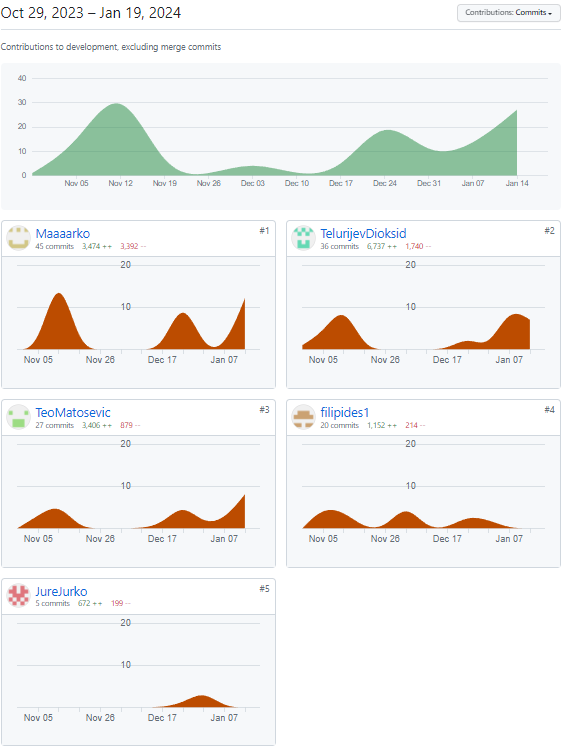
\includegraphics[scale=0.75]{slike/bp-ui-contr.PNG} 
				\centering
				\caption{Bytepit-ui}
				\label{fig:bytepit-ui}
			\end{figure}
			
			\eject
			
			\item \textbf{bytepit-api}
			
			\begin{figure}[H]
				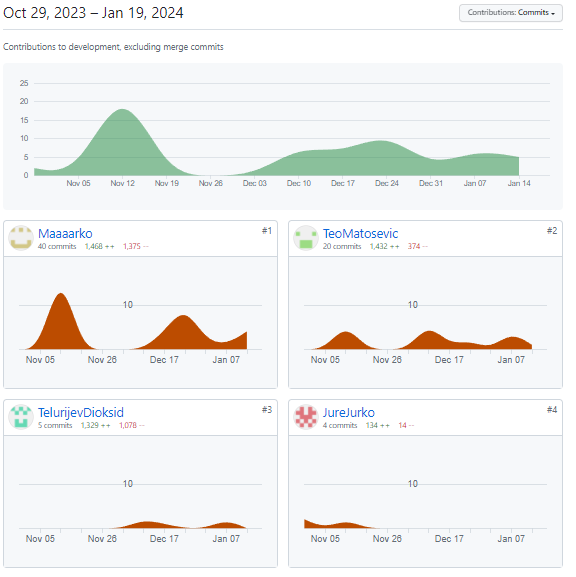
\includegraphics[scale=1.0]{slike/bp-api-contr.PNG} 
				\centering
				\caption{Bytepit-api}
				\label{fig:bytepit-api}
			\end{figure}
			
			\eject
			
			\item \textbf{bytepit-root}
			
			\begin{figure}[H]
				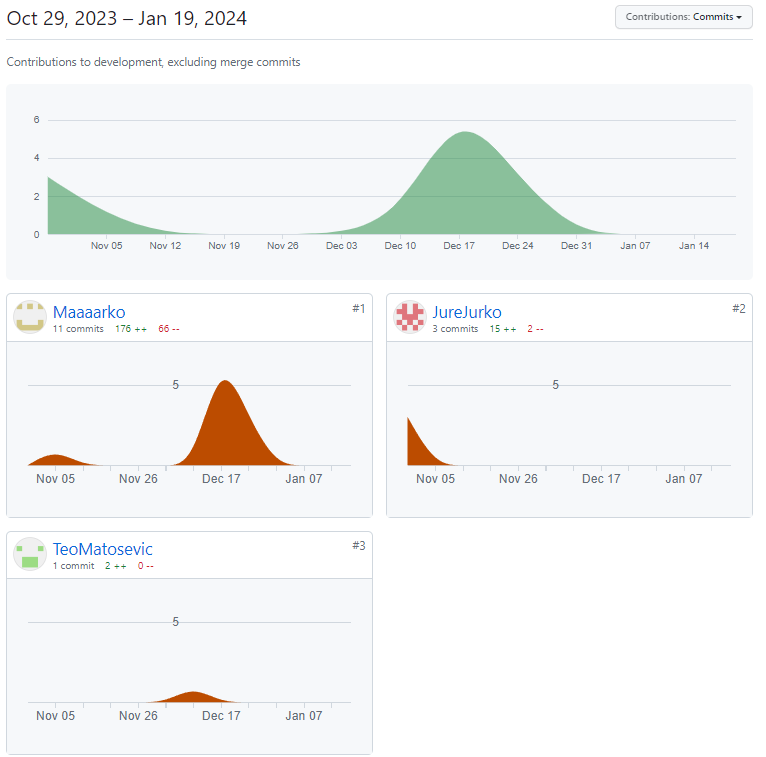
\includegraphics[scale=0.9]{slike/bp-root-contr.PNG} 
				\centering
				\caption{Bytepit-root}
				\label{fig:bytepit-root}
			\end{figure}
		\end{packed_enum}
		
		  
		
	


\end{document} %naredbe i tekst nakon ove naredbe ne ulaze u izgrađen dokument 


